\begin{figure}[htp]

\begin{subfigure}{\textwidth}
\begin{subfigure}{0.45\textwidth}
\centering
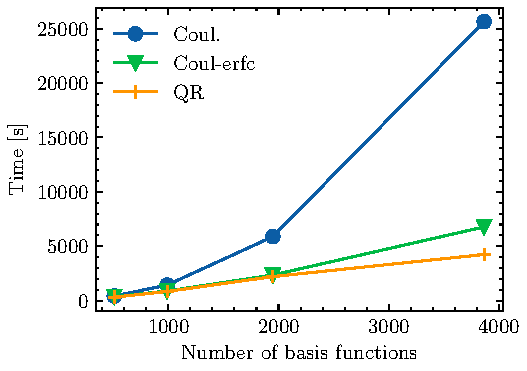
\includegraphics[width=\textwidth]{../articles/art2/adctime_acid}
%\captionof{figure}[This Figure]{Figure}
\end{subfigure}
\hfill
\begin{subtable}{0.45\textwidth}
\centering
\begin{tabular}{rrrr}
\hline
N$_{AO}$ & DFCM & DFCAM & QRDF \\ \hline
508 & --- & --- & --- \\ 
988 & 1.8 & 1.4 & 1.5 \\ 
1948 & 2.1 & 1.5 & 1.4 \\ 
3868 & 2.2 & 1.5 & 1.0 \\
 \hline
\end{tabular}
%\captionof{table}[This Table]{REDO THIS!!!!}
\end{subtable}
\caption{}
\label{fig:ES_TIME_LCA}
\end{subfigure}

\vspace{1.5\baselineskip}

\begin{subfigure}{0.45\textwidth}
\centering
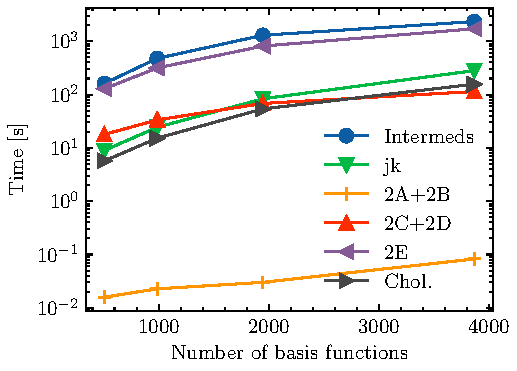
\includegraphics[width=\textwidth]{../articles/art2/adcsingle_acid}
\caption{}
\label{fig:ES_TIMESINGLE_LCA}
\end{subfigure}
\hfill
\begin{subfigure}{0.45\textwidth}
\centering
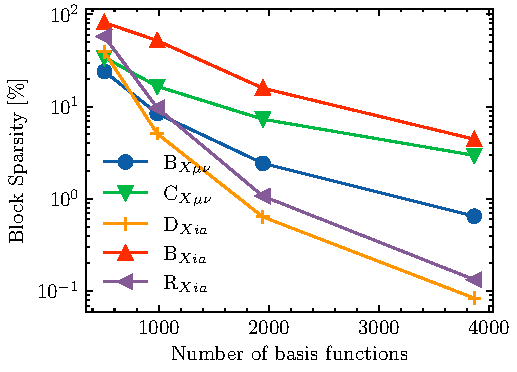
\includegraphics[width=\textwidth]{../articles/art2/blocksparsity_acid}
\caption{}
\label{fig:ES_SPARSITY_LCA}
\end{subfigure}

\caption{(a) Scaling behavior for the computation of a single matrix-vector-product with a CIS optimized (singlet) trial vector (LCA). (b) Total time needed to evaluate each separate component of the MVP using quasi-robust density fitting (LCA). (c) Block sparsity for the major 3-index tensors appearing in the evaluation of the MVP (LCA).}

\end{figure}

\begin{figure}

\begin{subfigure}{\textwidth}
\begin{subfigure}{0.45\textwidth}
\centering
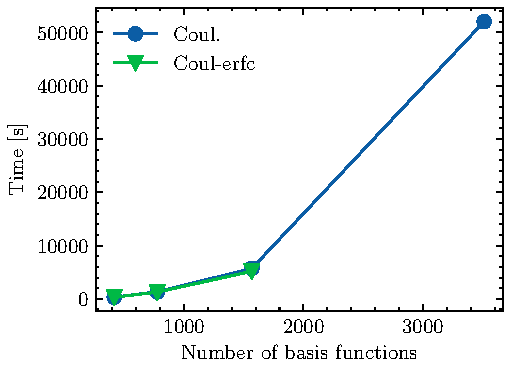
\includegraphics[width=\textwidth]{../articles/art2/adctime_fw}
%\captionof{figure}[This Figure]{Figure}
\end{subfigure}
\hfill
\begin{subtable}{0.45\textwidth}
\centering
\begin{tabular}{rrr}
\hline
N$_{AO}$ & DFCM & DFCAM \\ \hline
508	& ---	& --- \\
988	& 2.3	& 2.3 \\
1948 & 	2.1 &	2.0 \\
3868	 & 2.74 & --- \\
 \hline
\end{tabular}
\end{subtable}
\caption{}
\label{fig:ES_TIME_FW}
\end{subfigure}

\vspace{1.5\baselineskip}

\centering
\begin{subfigure}{0.45\textwidth}
\centering
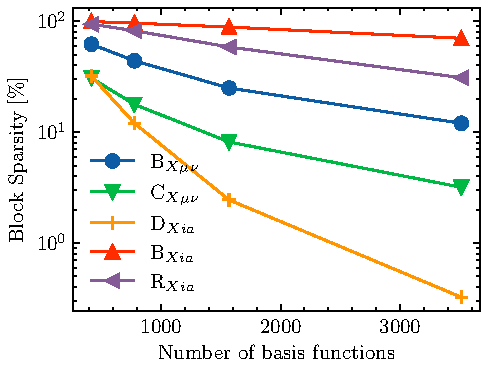
\includegraphics[width=\textwidth]{../articles/art2/blocksparsity_fw}
\caption{}
\label{fig:ES_SPARSITY_FW}
\end{subfigure}

\caption{(a) Scaling behavior for the computation of a single matrix-vector-product with a CIS optimized (singlet) trial vector (FW). (b) Block sparsity for the major 3-index tensors appearing in the evaluation of the MVP (FW)}

\end{figure}